\documentclass{article}
\usepackage{setspace}
\usepackage[top=1in, bottom=1.5in, left=1.25in, right=1.25in]{geometry}
\usepackage{booktabs}
\usepackage{graphicx}
\usepackage{caption}
\usepackage{amsmath}
\usepackage{subfigure}
\title{A HAR-DRD implementation using low-frequency OHLC candlestick data.}
\author{Heeth Surana}
\begin{document}
\doublespacing
\maketitle
\begin{abstract}
    A new approach to the HAR-DRD model is developed using lower frequency 
    daily candlestick price (Open, High, Low, Close) data. Contrary to using 
    a noisy and expensive measure for daily realized volatility with squared intraday
    returns sampled at high frequency, we employ an alternative estimator for daily realized volatility that 
    only uses daily candlestick prices. Additionally, daily correlation estimation and forecasting is
    replaced by weekly correlation forecasts on a daily rolling basis, in favor of producing less noisy and more stable
    correlation forecasts. The model is calibrated (2002-2017) and tested (2018-2022) in the context of a portfolio of four assets:
    US 10-Year Treasuries, US SP 500 Index, WTI Crude Oil, and Gold. Evaluation of out-of-sample forecasting errors show
    the model is reasonably stable across time. Testing the model in a minimum variance portfolio optimization problem
    yields favorable portfolio outcomes.
\end{abstract}
\section{Introduction}


Covariance forecasting has important implications in 
risk management and asset allocation problems, but they yet remain
challenging to model and forecast. While volatilies are relatively easier
to model, the correlation components of covariances are major contributors 
to this challenge. Over the last two decades, there has been considerable 
innovation in modeling volatilies and correlations (covariances).

One of the most popular traditional models in 
estimating and forecasting covariances was pioneered 
by Engle (2002)\cite{Engle2002} through their GARCH-DCC model. This 
entailed splitting the covariance matrix into the 
diagonal volatility matrix and a full-rank 
symmetrical correlation matrix. The asset volatilities 
are modeled using a GARCH process and the correlations 
are modeled using a GARCH-type DCC process.

Corsi (2009)\cite{Corsi2009} developed a simpler yet effective model to 
estimate single asset volatilities with an AR-style Heterogenous Auto Regressive (HAR) model. 
Muller's (1997)\cite{Muller1997} 'Heterogenous Market 
Hypothesis' theorizes that the market is composed of non-homegenous parties that differ
in terms of investment objectives and trading appetite. Corsi (2009) augmented this idea by
suggesting that daily volatility is a function of volatility cascades observed at various frequencies,
wherein each heterogenous investor group is uniquely contributing to daily volatility.
Specifically, Corsi (2009) proposed that daily volatility can 
be modeled as a linear function of past realized 
volatilies observed at the daily, weekly, and monthly 
intervals. 

Corsi's (2009) univariate HAR model was extended to a 
mutlivariate setting to directly model covariances via the 
Cholesky decomposition on the covariance matrix by 
Chiriac and Voev (2011)\cite{Chiriac2011}. Oh and Patton (2016)\cite{OhPatton2016} and 
Bollerslev et al. (2018)\cite{Bollerslev2018} developed an alternative approach
to use the HAR in modeling covariances. Similar to 
Engle's (2002) approach, the covariance matrix is 
decomposed into volatilies and correlations components 
(DRD), which are then modeled using two separate 
multivariate HAR models instead of directly modeling covariances. 
They use a parsimonious specification by vectorizing the matrices,
thus applying just one set of HAR parameters to model all asset volatilies
and pairwise correlations respectively. This allows easy estimation of model
parameters regardless of the dimensions of the covariance matrix.   
They noted that their HAR-DRD implementation outperforms the HAR-Cholesky.

Symitsi et al. (2018)\cite{Symitsi2018} compared forecasting performance of the
Vectorized HAR-DRD model, similar to Oh and Patton's (2016) implementation,
against a fully Generalized HAR-DRD Model that allows each variance-covariance term
to be modeled by its own dynamics, significantly increasing the number of estimated parameters. Testing in the context of a portfolio of 
major European equity indices, they concluded the Vector HAR-DRD produces more favourable 
losses in out-of-sample fit in most cases while also providing superior parsimony and 
ease of computation.  Moreover, they also tested the Vectorized HAR-DRD model's performance against
other popular covariance forecasting models with GARCH and MA-type specifications. 
They concluded that the Vector HAR-DRD model outperformed all 
competing models in producing the best out-of-sample fit based on matrix norm calculations.

The use of high frequency data is quite often the source of HAR's clear advantage over
competing models in volatility as well as covariance forecasting. Implementations often make use of tick level or 5-minute interval data.
Daily volatility is typically estimated by averaging squared returns over the chosen number of 
intraday intervals. Daily correlations are also estimated using high frequency intraday data. 
However, Bollerslev and Andersen (1998)\cite{Bollerslev1998} note that intraday returns at such frequencies are extremely noisy, and are 
also prone to measurement errors due to market microstructure
effects. Furthermore, sourcing data at such frequencies is an expensive exercise.

Alternative estimators of daily realized volatility using lower frequency data have been used, albeit few.
In one example, Engle and Gallo (2006)\cite{Engle2006} employ an estimator for daily volatility using
the daily log-range estimator, which simply takes the log
difference of the daily high and daily low as a variance proxy. Several better estimators exist, 
but have not been brought into popular use with HAR models.

For instance, Parkinson (1980)\cite{Parkinson1980} proposed a more efficient and unbiased variance
measure by squaring the log difference of high and low prices,
and scaling them by $\frac{1}{4\ln{2}}$. Garman and Klass (1980)\cite{Garman1980} suggested a measure that also incorporates
opening and closing prices. Both estimators offer an unbiased 
measure of variance when data is continuously sampled, although 
they assume zero drift in returns. This assumption is unlikely 
empirically. To combat this, Rogers and Satchell (1991)\cite{Rogers1991} proposed 
an alternative drift-independent unbiased measure which also takes open 
and close prices in addition to the high and low prices. All above
measures are subject to a downward bias problem when applied to
actual data. Yang and Zhang (2000)\cite{Yang2000} offer correction methods but
are often impractical since they either require parameters that are 
not empirically available or require us to measure variances 
in a multi-period setting which is not fit for HAR models.

While estimators for volatility using lower frequency data exist, a similar type
of proxy is difficult to develop for a daily correlation estimate. Rogers and Zhou (2008)\cite{Rogers2008} 
attempted to devise such an estimate using daily candlestick data, but concluded that
while their measure is unbiased, it lacks any decisive advantages and dependability.

We propose an alternative HAR-DRD implementation that uses daily candlestick price data (Open, High, Low, Close)
in estimating daily realized volatility, and foregoes daily correlation measures by simply forecasting over 
a weekly horizon. We theorize that this method offers a simple solution to reduce the implications
of noisy intraday returns data on forecasts, and test its performance stability across time as well as outcomes 
in a portfolio optimization problem.
 











\section{Methodology}
\subsection{Data}
The HAR-DRD model's implementation and testing is in the context of a portfolio of four assets: US 10-Year Treasury, US SP500, WTI Crude Oil, and Gold. 
Price data for each security is extracted from its respective first generic futures contract from 2002 to 2022. The dataset is divided into 
training (January 2002- December 2017) and testing(January 2018- December 2022) sets to calibrate and evaluate the model respectively. Figure 1 shows the cumulative 
returns of the assets in the period.\footnote{Negative Crude Oil Prices in 2020 have been modified as close to 0 for ease of modeling.}

\begin{figure}[ht]
    \centering
    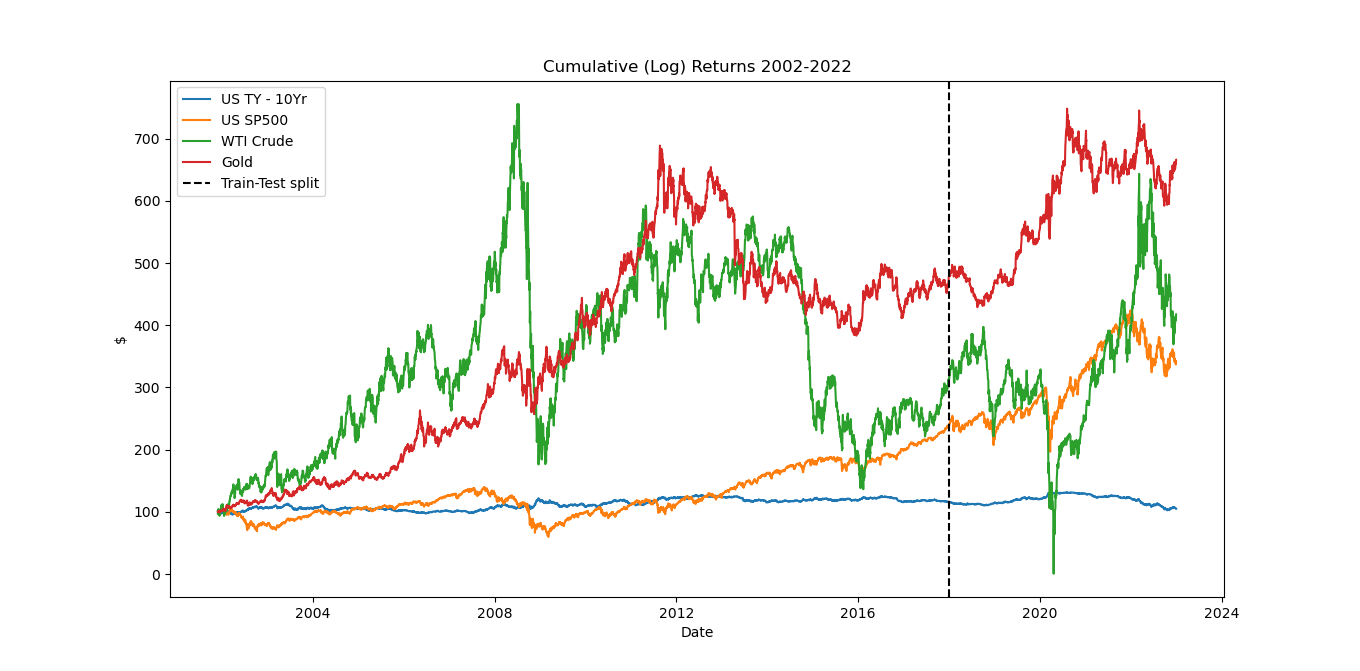
\includegraphics[width=0.8\textwidth]{"Figures/Cumulative Asset Returns.png"} 
    \captionsetup{width=0.7\textwidth,justification=centering}
    \caption{Cumulative Asset Returns based on \$100 starting value. 2002-2018 data is
    used for model training, which is tested on returns data from 2018-2022.}
    \label{fig:my_image}
\end{figure}


Typically, HAR implementations have been studied in the context of
single assets or multiple assets of similar types, such as an all-equity portfolio. It is worthwhile to observe the HAR model's performance
for a portfolio composed of assets that exhibit much more varied distributional properties. For this purpose, securities from unique asset classes are chosen.
Table 1 summarises key summary statistics for each asset during the period (2002-2022).

WTI Crude Oil returns particularly exhibit a significant departure in their distribution parameters compared to
the rest, with heavier tails, a wider spread,  and more extreme negative skew. It is likely that the 2020 Oil Price Shock is a major
contributor in these.

We also see reasonable variety in distributional features of other securities. For instance, treasuries exhibit a relatively tight
distribution. US SP500 and Gold have comparable spread and skew, although SP500 exhibits heavier tails.
\begin{table}[ht]
    \centering
    \caption{Descriptive statistics of daily asset returns 2002-2022}
    \begin{tabular}{lcccc}
    \toprule
    \textbf{Security} & \textbf{Mean} & \textbf{Std. Dev.} & \textbf{Skew} & \textbf{Kurtosis} \\
    \midrule
    US 10-Year Treasury & 10e-5 & 3.85e-3 & -0.22 & 4.25 \\
    US SP500 & 2.33e-4 & 1.25e-2 & -0.35 & 12.79 \\
    WTI Crude Oil & 2.71e-4 & 9.9e-2 & -8.42 & 2309.43 \\
    Gold & 3.6e-4 & 1.1e-2 & -0.36 & 5.20 \\
    \bottomrule
    \end{tabular}
    \label{tab:descriptive_stats}
    \end{table}


\subsection{HAR-DRD specification}

Similar to Oh and Patton's (2016) implementation, the covariance matrix ($\Sigma$) can be 
decomposed into a diagonal volatilies matrix (D) and a symmetrical correlations matrix (R).
In a portfolio of four assets, this can be visualized as follows:

\begin{equation*}
    \Sigma =
    \begin{bmatrix}
        \sigma_1 & 0 & 0 & 0 \\
        0 & \sigma_2 & 0 & 0 \\
        0 & 0 & \sigma_3 & 0 \\
        0 & 0 & 0 & \sigma_4 \\
    \end{bmatrix} 
    _{\substack{\text{D}}}
    \quad
    \begin{bmatrix}
        1 & \rho_{1,2} & \rho_{1,3} & \rho_{1,4} \\
        \rho_{1,2} & 1 & \rho_{2,3} & \rho_{2,4} \\
        \rho_{1,3} & \rho_{2,3} & 1 & \rho_{3,4} \\
        \rho_{1,4} & \rho_{2,4} & \rho_{3,4} & 1 \\
    \end{bmatrix}
    _{\substack{\text{R}}}
    \quad
    \begin{bmatrix}
        \sigma_1 & 0 & 0 & 0 \\
        0 & \sigma_2 & 0 & 0 \\
        0 & 0 & \sigma_3 & 0 \\
        0 & 0 & 0 & \sigma_4 \\
    \end{bmatrix}
    _{\substack{\text{D}}}
\end{equation*}

This separation allows for the modeling of volatilies and correlations with separate parameters. 
The HAR model specification for volatilies can be shown as:

$$\sigma_{i,t+1}^{(d)} = c + \beta^{(d)}RV_{i,t}^{(d)} + \beta^{(w)}RV_{i,t}^{(w)} + \beta^{(m)}RV_{i,t}^{(m)} + \epsilon_{i,t+1}^{(d)},$$
$$  i = 1,2,3,4 $$

where RV is the daily realized volatility; and \textit{d}, \textit{w}, and \textit{m} denote daily,
weekly, and monthly frequencies respectively. The coefficents (parameters)
are estimated using OLS, and $\epsilon$ is the error term. Note that the same set of parameters
are used to model volatilies across all assets. The number of parameters remain fixed
irrespective of the dimensions(number of assets), making this model scalable and parsimonious.

In implementations that use high-frequency intraday data, 
$ RV_{i,t}^{(d)} = \frac{1}{N}\sum_{k=1}^N r_{k,t}^2 $ where
N is the number of intraday subintervals. Returns that are sampled at high
values of N are often expensive to obtain, exhibit noisiness, and
are prone to measurement errors.

An alternative measurement for daily realized volatility by Rogers and Satchell (1991) is used in our
implementation. This estimate uses daily candlestick data to produce an unbiased and
drift-independent measure of daily volatility. This alternative estimator is defined as follows:

$$ RV_{i,t}^{(d)} = \sqrt{u_{i,t}(u_{i,t} - c_{i,t}) + d_{i,t}(d_{i,t} - c_{i,t})},$$
$$u_{i,t} = \ln H_{i,t} - \ln O{i,t}$$
$$d_{i,t} = \ln L_{i,t} - \ln O{i,t}$$
$$c_{i,t} = \ln C_{i,t} - \ln O{i,t},$$ 
$$  i = 1,2,3,4 $$

Irrespective of the estimation method used for daily realized volatility, 
weekly and monthly realized volatilies are simply daily volatilies
averaged across their respective frequencies:
$$RV_{i,t}^{(w)} = \frac{1}{5} \sum_{k=0}^4 RV_{i,t-k}^{(d)} $$
$$RV_{i,t}^{(m)} = \frac{1}{21} \sum_{k=0}^{20} RV_{i,t-k}^{(d)} $$


Typical HAR-DRD implementations model correlations on a daily horizon using
high-frequency intraday data. In such implementations, the daily correlation 
is modeled in an almost similar fashion to volatilities:
$$vech(R_{t+1}) = vech(\bar{R}_T)(1 - \alpha - \beta - \gamma) + \alpha\cdot vech(R_{t}) + \beta\cdot vech(R_{t-4:t}) + \gamma\cdot vech(R_{t-20:t})+ vech(\epsilon_{t+1}),$$

where the \textit{vech} operator signifies a vectorized form of the lower-triangular
correlation matrix (R). Correlations on a given day are modeled as a linear
function of correlations observed over the previous day, previous week, previous month,
and a long-term time period \textit{T} (for example: average correlation observed over last 10 years).

Reiterating the noisiness of intraday returns, correlations are likely to be noisy and 
oscillate when measuring on a daily basis. In a portfolio optimization application, such
approaches are not so ideal since they are likely to cause portfolio weights to 
shift excessively on a daily basis, making daily rebalancing unviable.

We propose an alternative, simpler approach which estimates correlation on a daily basis, but over
a weekly horizon. In other words, on any given day, the model is forecasting the correlations
that are to be observed in the following week. Since the lowest frequencies that are incorporated
in this model are weekly versus the daily in the typical implementation, correlation measures are 
likely to be less noisy and more stable. This alternative specification is described as follows:
$$vech(R_{t+1:t+5}) = vech(\bar{R}_T)(1 - \alpha - \beta) + \alpha\cdot vech(R_{t-4:t}) + \beta\cdot vech(R_{t-20:t}) + vech(\epsilon_{t+1:t+5}),$$

where weekly correlations are modeled on a daily rolling basis, as a function of correlations observed
during the past week, past month, and a long-term time period \textit{T}. Coefficents are similarly estimated using OLS,
and are singularly applied to all pairwise correlations, maintaining parsimony.

\section{Results}
\subsection{Model Parameters}

OLS regression results for both volatility and correlation models
return statistically significant coefficents. The results are summarized in
Table 2 and Table 3 resepctively.

\begin{table}[ht]
    \centering
    \caption{Regression results for volatilties}
    \begin{tabular}{lcccc}
    \toprule
    \textbf{} & \textbf{Coeff} & \textbf{Std. Err.} & \textbf{[0.025} & \textbf{0.075]} \\
    \midrule
    c & 0.00 & 0.00 & 0.00 & 0.00 \\
    $\beta^{(d)}$ & 0.15 & 0.01 & 0.13 & 0.17 \\
    $\beta^{(w)}$ & 0.38 & 0.02 & 0.34 & 0.41 \\
    $\beta^{(m)}$ & 0.43 & 0.02 & 0.40 & 0.46 \\
    \bottomrule
    \end{tabular}
\end{table}

\begin{table}[ht]
    \centering
    \caption{Regression results for correlations}
    \begin{tabular}{lcccc}
    \toprule
    \textbf{} & \textbf{Coeff} & \textbf{Std. Err.} & \textbf{[0.025} & \textbf{0.075]} \\
    \midrule  
    $\alpha$ & 0.05 & 0.00 & 0.03 & 0.06 \\
    $\beta$ & 0.40 & 0.01 & 0.38 & 0.43 \\  
    \bottomrule
    \end{tabular}
\end{table}

A consistent observation across both regression results is that the lower frequency
variables have a stronger contribution to daily volatilies and weekly correlations. 
This suggests that both volatility and correlation exhibit persistence in general.

\subsection{Out-of-sample losses in fit}

Forecasted daily volatilies and weekly correlations were compared to actual observations
in the test period (2018-2022), to test for homescedastic errors and model stability across
the forecasting period (2018-2022). Volatility forecast errors were measured using the Euclidean distance ($L_2$ norm)
between the actual and forecasted vectorized volatility diagonal matrices. Similarly, correlation forecast
errors were measured using the $L_2$ norm between the actual and forecasted vectorized correlation matrices.

The results for both are graphed in Figure 2 and Figure 3, respectively.

\begin{figure}
    \centering

    \subfigure[Pre 2020 Oil Crash]{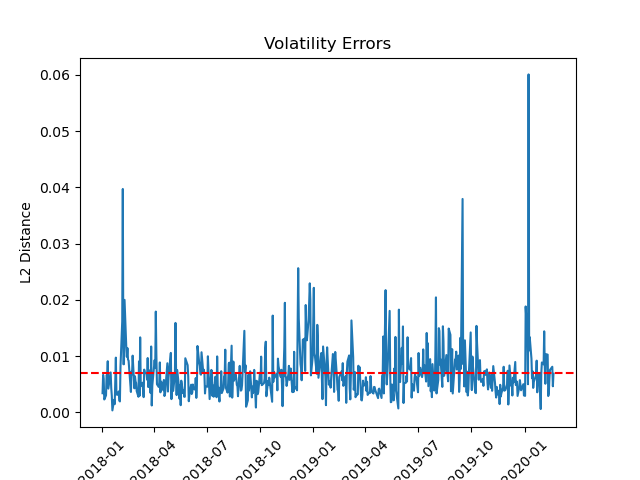
\includegraphics[width=0.8\textwidth]{"Figures/VolatilityLoss_PreOilCrash.png"}}
    \subfigure[Oil Crash]{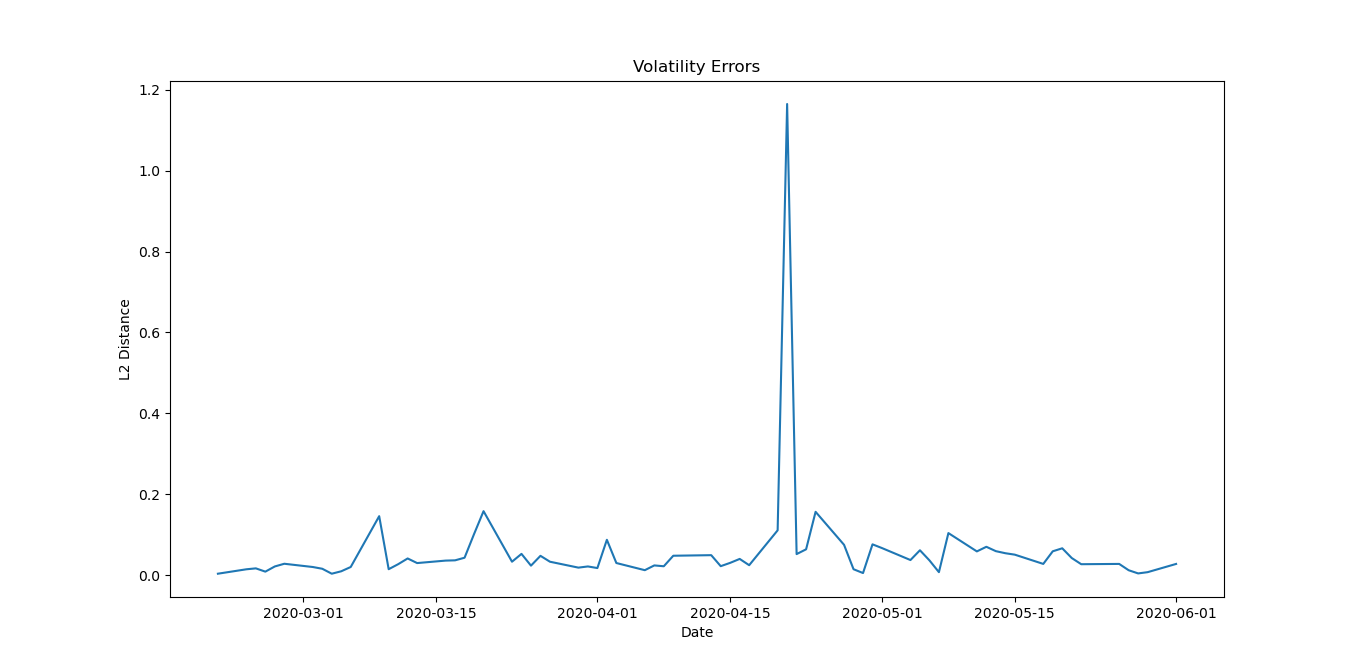
\includegraphics[width=0.8\textwidth]{"Figures/VolatilityLoss_OilCrash.png"}}
    \subfigure[Post 2020 Oil Crash]{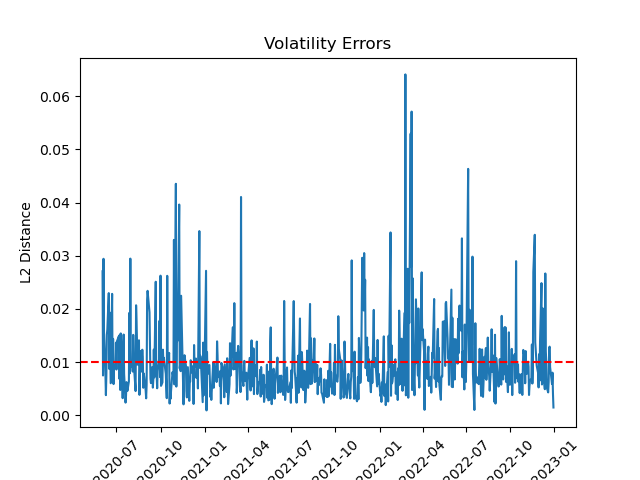
\includegraphics[width=0.8\textwidth]{"Figures/VolatilityLoss_PostOilCrash.png"}}
    \caption{Forecasting errors in volatilities (2018-2022)}
\end{figure}

We note that errors in volatility forecasts are generally stable, with spikes and troughs centred
around 0.01. The Oil Crash in the spring of 2020 caused a pronounced spike in the error (Figure 2 (b)), 
and the time period following the crash exhibits a relatively higher frequency in spikes (Figure 2 (c)) compared to
the pre oil crash period (Figure 2 (a)). Nevertheless the model errors revert back to hovering around
the long run average reasonably quickly without notable structural breaks.

\begin{figure}[ht]
    \centering
    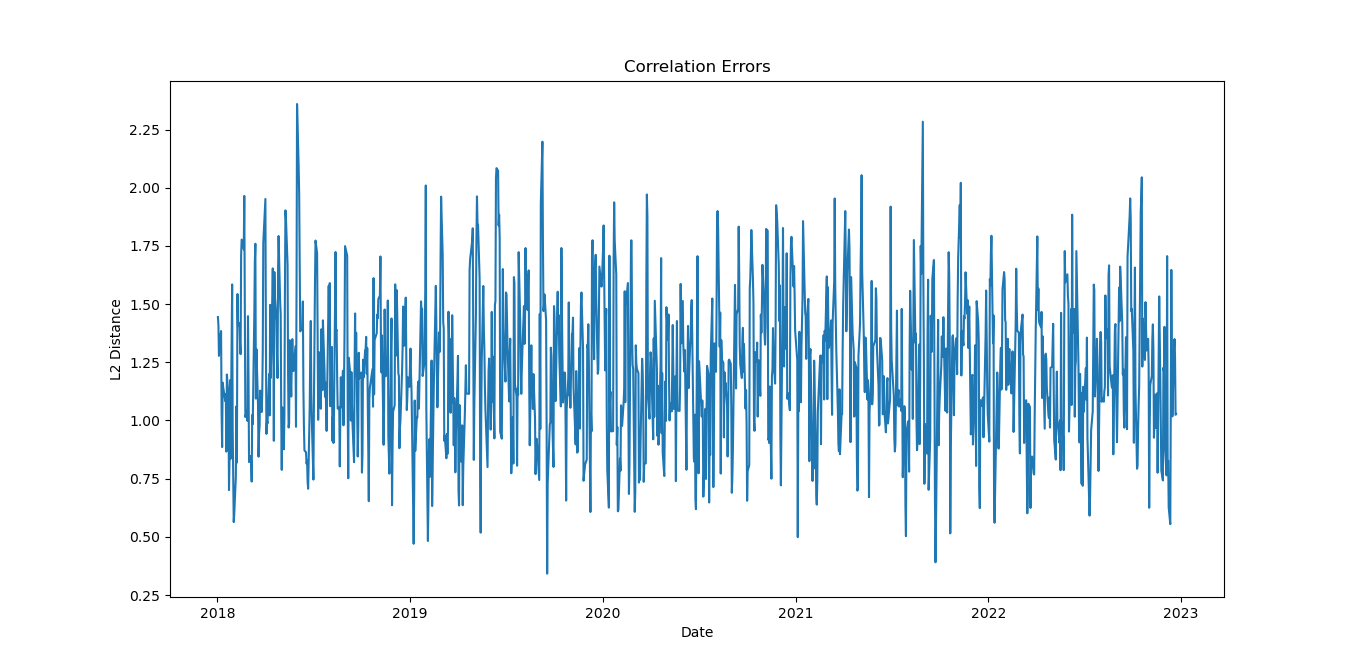
\includegraphics[width=0.8\textwidth]{"Figures/CorrelationLoss.png"} 
    \captionsetup{width=0.7\textwidth,justification=centering}
    \caption{Forecasting errors in correlations (2018-2022)}
\end{figure}


Stability in correlation forecasting errors is more straightforward. Errors consistently
oscillate at around 1.25 across the five years, suggesting a reasonable model response to shifting correlations across
regimes or time periods.

\subsection{Model performance in a portfolio optimization problem}

The HAR-DRD model's correlation and volatility forecasts were synthesized into covariance forecasts which were then used in a minimum-variance portfolio construction problem.
Its performance was compared against a baseline model that used historical (t-1) covariance to construct
portfolio weights. The historical model simply used volatilies from the previous day, and correlations that have been observed in the 
previous week. 

The optimization problem can be summarized as follows:

$$ Min \,\, \omega^T \Sigma \omega $$
$$ s.t.: \,\,\sum_{i=1}^n \omega_i = 1,\,\omega_i \ge 0, \forall_i,$$


where $\omega$ is the vector of portfolio weights and $\Sigma$ is the covariance matrix of asset returns.

Cumulative returns for both the HAR-DRD and the baseline historical model is graphed in Figure 4.
It is evident that the HAR-DRD produces favorable portfolio volatility outcomes. 

\begin{figure}[ht]
    \centering
    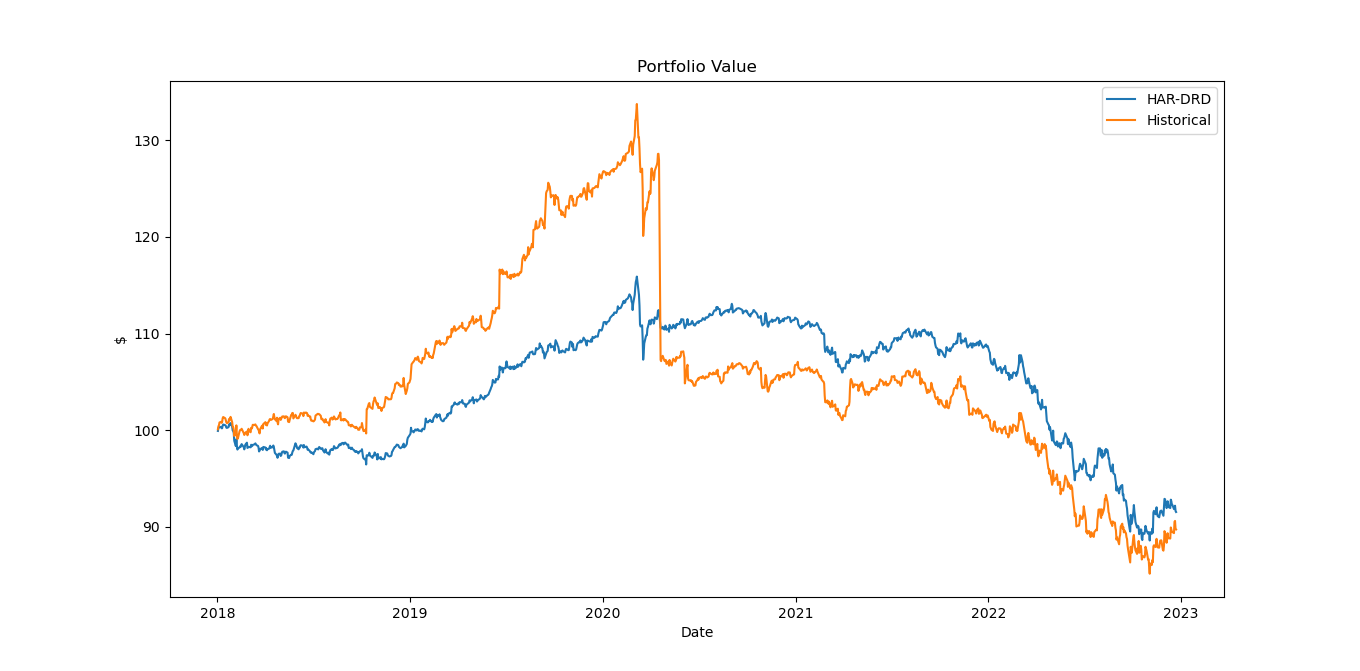
\includegraphics[width=0.8\textwidth]{"Figures/Portfolio_Value.png"} 
    \captionsetup{width=0.7\textwidth,justification=centering}
    \caption{Portfolio optimization outcomes for HAR-DRD vs historical approach, \$100 starting value}
\end{figure}

Table 4 summarizes this more comprehensively by reporting annualized volatility by year.  

\begin{table}[ht]
    \centering
    \caption{Annualized Portfolio Volatility (2018-2022)}
    \begin{tabular}{lcccc}
    \toprule
    \textbf{Year} & \textbf{HAR-DRD} & \textbf{Historical}  \\
    \midrule
    2018 & 0.03 & 0.05 \\
    2019 & 0.03 & 0.07 \\
    2020 & 0.05 & 0.19 \\
    2021 & 0.04 & 0.05 \\
    2022 & 0.08 & 0.10 \\
    \bottomrule
    \end{tabular}
\end{table}

The HAR-DRD consistently performs closer to the objective of minimizing portfolio
volatility compared to the baseline model. In particular, it successfuly protects 
portfolio volatility during the highly volatile 2020 fiscal year. We see marginally
higher volatilies in the HAR-DRD portfolio in 2021 and 2022 compared to 2018 and 2019, which is consistent with
our volatility forecast error observations from section 3.2. 


\section{Conclusion}

An alternative approach to HAR-DRD modelling is developed which uses daily candlestick data for volatilities
and foregoes daily correlations in favor of weekly correlations forecasts. We show that this is a viable model in the absence of high-frequency
intraday returns data. This method also has clear advantages to high-frequency
HAR implementations in terms of data noise and extraction costs.

We report that this modified approach produces a model that is reasonably stable across time periods 
and regimes, and produces favorable portfolio optimzation outcomes when compared to a simple
historical approach.

There are notable areas that can be futher explored in this research. It will be worthwhile to compare
this HAR-DRD model's performance against other models such as the traditional high-frequency HAR-DRD models,
and the GARCH-DCC model. Additionally, an interesting extension is to observe performance decay of this model
when we increase the forecasting horizon from daily to weekly and monthly. 

Moreover, innovations in other facets of the HAR model can be interesting to attempt. One possible direction
is to make the parameters of the HAR model time-varying, or alternatively employ hidden markov models to 
estimate parameters that are unique to each market regime. 
\newpage
\bibliographystyle{plain}
\bibliography{references}
\end{document}